\documentclass[class=article, crop=false]{standalone}
\usepackage[subpreambles=true]{standalone}
\usepackage{import}
\usepackage[T1]{fontenc}
\usepackage[utf8]{inputenc}
\usepackage[english, danish]{babel}
\usepackage{graphicx,wrapfig,lipsum}

\begin{document}
    Nedenstående Figur~\ref{fig:use_case_model}  er et use-case diagram, der præsenterer de forskellige use cases og deres relationer til spilleren, samt deres indbyrdes sammenhæng. Det blev besluttet at opdele, hvad der kunne have været én stor use case (som nok ville kaldes, “Spil spillet”) op i flere use cases, for bedre overblik over programmets forskellige elementer.
    \begin{figure}[H]
        \centering

        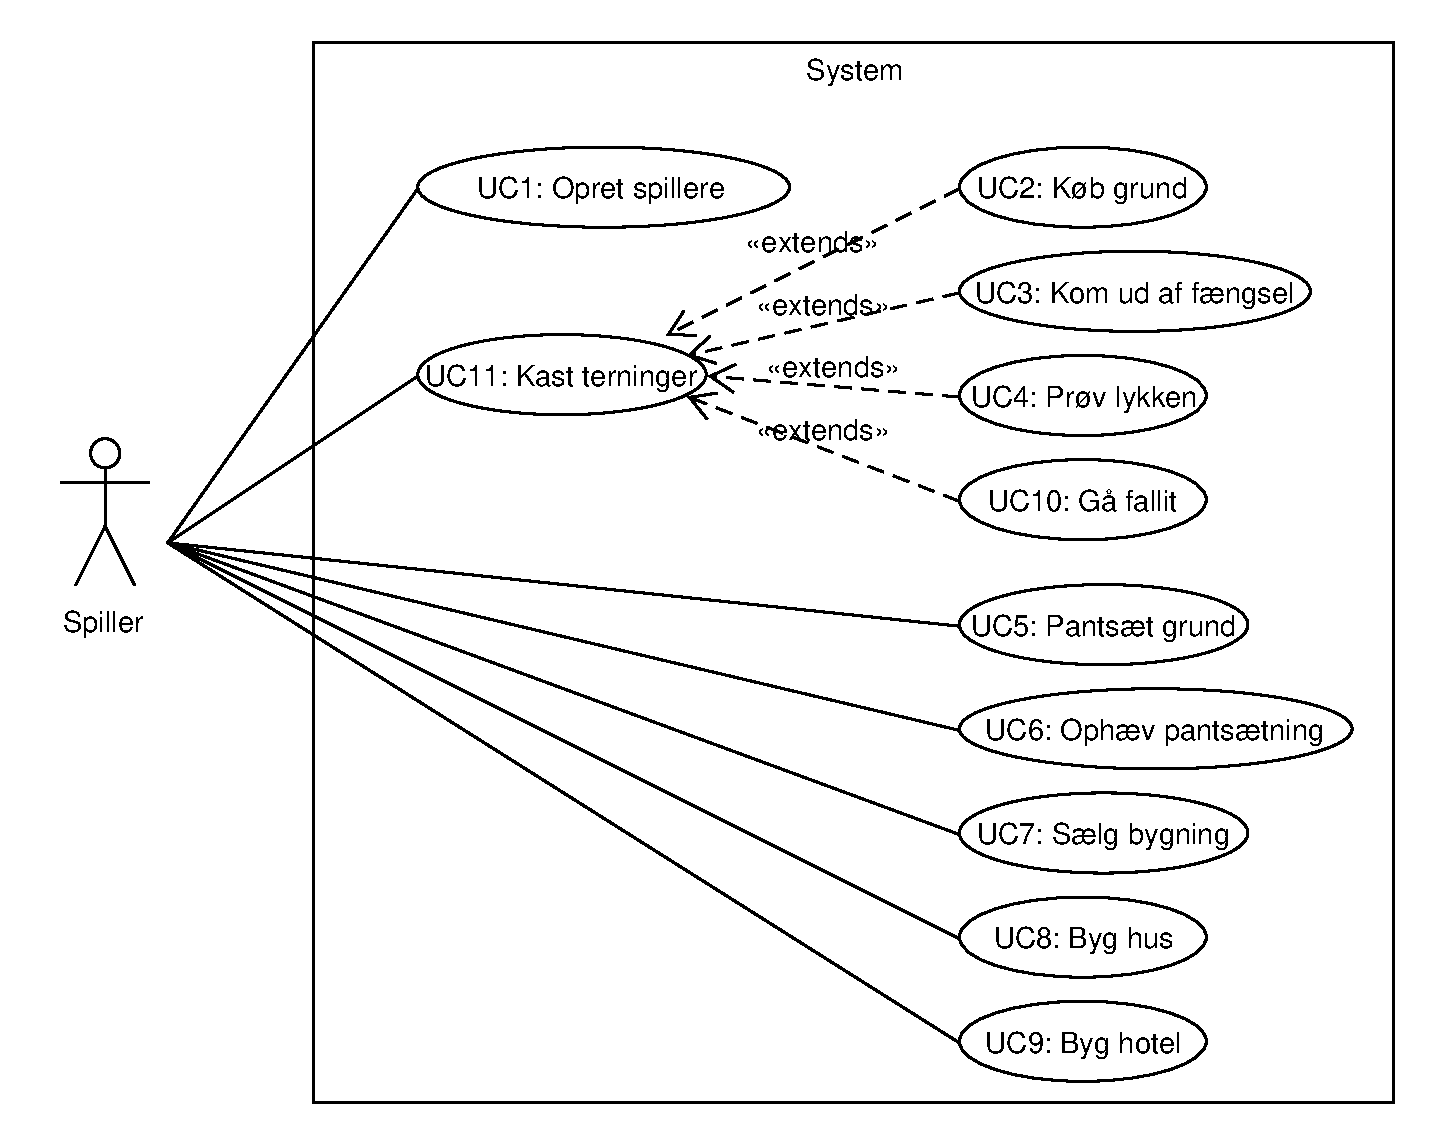
\includegraphics[scale=0.7]{diagrams/use_case_diagram.pdf}
        \caption{Use case diagram over systemet}\label{fig:use_case_model}
    \end{figure}

    I næste afsnit er de enkelte use cases mere mere detaljeret beskrevet for sig selv, i use case beskrivelser.

\end{document}